\documentclass{article}
\usepackage[final]{proposal_style}
\usepackage[utf8]{inputenc} % allow utf-8 input
\usepackage[T1]{fontenc}    % use 8-bit T1 fonts
\usepackage{hyperref}       % hyperlinks
\usepackage{url}            % simple URL typesetting
\usepackage{booktabs}       % professional-quality tables
\usepackage{amsfonts}       % blackboard math symbols
\usepackage{nicefrac}       % compact symbols for 1/2, etc.
\usepackage{microtype}      % microtypography
\usepackage{graphicx}
\usepackage[many]{tcolorbox}
\usepackage{trimclip}
\usepackage{listings}
\usepackage{multicol}
\usepackage{environ}% http://ctan.org/pkg/environ
\usepackage{wasysym}
\usepackage{array}
\newcommand{\Checked}{{\LARGE \XBox}}%
\newcommand{\Unchecked}{{\LARGE \Square}}%
\setcitestyle{square}
\pagenumbering{gobble}

\title{CS 475/675 Project Proposal}
% TODO replace with your project title

\author{
  Rupsa Acharya, Rishima Mukherjee, Harrison Khoo, Dimitri Lezcano\\
  rachary6, rmukher9, hkhoo2, dlezcan1
  % TODO replace with your names and JHEDs
}

\begin{document}
\maketitle

\begin{abstract}
We propose a model to characterize small molecules as potential inhibitors of Epidermal Growth Factor Receptor (EGF), a protein upregulated in cancer cells. We will compare neural network and random forest models to determine which molecular fingerprints are good indicators of protein inhibition.
% TODO write a two sentence abstract
\end{abstract}

\section{Project choice}

Choose either a {\bf methods} or {\bf applications} project, and a subarea from the below table.
\begin{table}[!h]
\centering
\def\arraystretch{2}
\begin{tabular}{c c c c c }
\toprule
% TODO replace "\Unchecked" with "\Checked" to choose an Applications project
\multicolumn{5}{l}{\Checked \bf Applications} \\
% TODO replace "\Unchecked" with "\Checked" on one of the five options below to choose that type of Applications project
\Checked Genomics data & 
\Unchecked Healthcare data & 
\Unchecked Text data &
\Unchecked Image data &
\Unchecked Finance data \\
\midrule
% TODO replace "\Unchecked" with "\Checked" to choose an Methods project
\multicolumn{5}{l}{\Unchecked \bf Methods} \\
% TODO replace "\Unchecked" with "\Checked" on one of the five options below to choose that type of Methods project
\Unchecked Fairness in ML &
\Unchecked Interpretable ML &
\Unchecked Graphical Models &
\Unchecked Robust ML &
\Unchecked Privacy in ML \\
\bottomrule
\end{tabular}
\end{table}

\section{Introduction}
Epidermal Growth Factor Receptor (EGF) is a protein critical to cell division signalling pathways. EGF is often overexpressed in cancerous cells, resulting in rapid cell division and cancer proliferation. Thus, EGF is a common therapeutic target to slow down or stop cancer proliferation. The dataset we are working with distinguishes small molecules as inhibitors or not an inhibitor for eight signalling pathways with well known roles in cancer progression; we will focus on the approximately 6,000 samples that assess the molecules as inhibitors for the EGF kinase. The input for each molecule is 8192 binary features/fingerprints associated with each molecule. We will use two models to train and classify small molecules as inhibitors for the EGF pathway. Our primary model is a neural network and we shall use a secondary, random forest model as a comparison. We will output a prediction determining whether a specific molecule is an inhibitor to the EGF kinase.

\section{Dataset and Features}
The provided training and test datasets on Kaggle have 6055 and 882 small molecule inhibitor candidates, respectively, associated with EGFR~\cite{inhibitordataset}. For each small molecule, there is an inhibitor label and 8192 features/fingerprints that comprise the small molecule characteristics. As is, the small molecules and fingerprints are unlabeled. We will retrieve the molecule IDs using provided h5 files with similar data. The fingerprint IDs are nonsensical integers, so we will use a more standard numbering system in its place. Additionally, we hope to reduce the number of input features into the model, so we will perform principal component analysis to extract fingerprints of note.

\begin{figure}
    \centering
    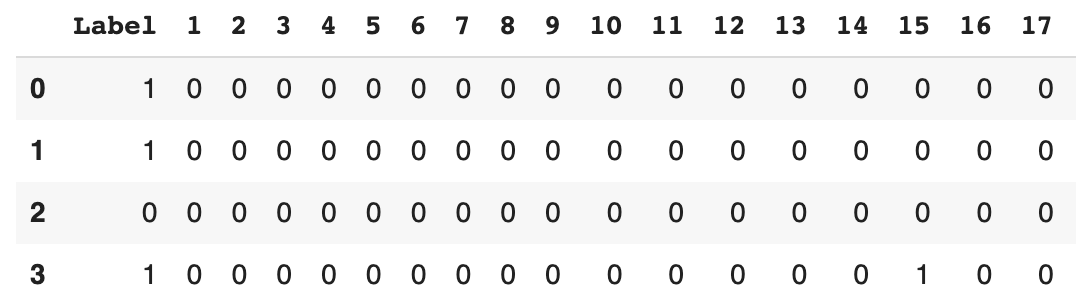
\includegraphics[width=18cm]{Data.png}
    \caption{Example of small molecule fingerprints from Kaggle}
    \label{}
\end{figure}

\newpage

\section{Methods}
We plan to use a feed-forward neural network to perform the classification of the molecular fingerprints to classify whether the molecule is a cancer inhibitor or not. Our model’s hypothesis class will be the set of functional compositions of linear transforms followed by a non-linear activation (most likely ReLU). Our loss function will be Class-weighted focal cross-entropy as we have seen from the dataset that there exists a label imbalance between the non-inhibitors and inhibitors~\cite{cui2019classbalanced}. This loss allows for the rebalancing of weights associated to the loss of misclassified samples dependent upon the number of samples that are present in the training dataset. The optimization we plan on using is batch gradient descent using the Adam optimizer. Adam optimization is selected for its good performance on stochastic gradient descent, allowing for efficient optimization~\cite{kingma2017adam}.

Furthermore, we plan to use random forest classification as an alternative learning method. The loss function we intend to use is Gini impurity as a measure of misclassification and will optimize our random forest classification by using a random sampled grid-search method over the parameters of the random forest classifier. The parameters that will be optimized will be: tree’s max depth, tree’s minimum samples to split, and the tree’s minimum number of leaf nodes. 



\section{Deliverables}
These are ordered by how important they are to the project and how thoroughly you have thought them through. You should be confident that your ``must accomplish'' deliverables are achievable; one or two should be completed by the time you turn in your Nov 19 progress report.

\subsection{Must accomplish}

\begin{enumerate}
\item Exploratory data analysis: feature and class distribution, correlations, etc.
\item Feature engineering and feature selection
\item Trained neural network model to predict effectiveness of small molecule better than random classification.
\item Compare neural network performance to random forest method.

\end{enumerate}

\subsection{Expect to accomplish}

\begin{enumerate}
    \item Achieve 75\% accuracy with neural network model
    \item Hyper-parameter tuning of neural network model for best performance
    \item Compute neural network model performance metrics (accuracy, sensitivity, specificity, precision, recall, \textbf{F1 score})
\end{enumerate}

\subsection{Would like to accomplish}

\begin{enumerate}
    \item Achieve 85\% accuracy with neural network model
    \item State of the art accuracy achieved.
    \item Evaluate our neural network model on external, unlabeled PubChem dataset and validity of predictions with literature search

\end{enumerate}

% \section*{References}
% \small
% TODO replace these with your citations. These are just examples.
% [1] https://www.kaggle.com/xiaotawkaggle/inhibitors
% \nocite{*}
\bibliographystyle{IEEETran}
\bibliography{Reflist}



\end{document}